\documentclass[10pt]{beamer}

% ------------------------------------------------------------------------
% Carga del preámbulo personalizado
% (Recuerda colocar tu archivo preamble.tex en la misma carpeta,
%  con definiciones de temas, colores, macros, etc.)
% ------------------------------------------------------------------------
\usetheme[progressbar=frametitle]{metropolis}
\usepackage{appendixnumberbeamer}
\usepackage{fancyvrb}
\usepackage{booktabs}
\usepackage[scale=2]{ccicons}
\usepackage{pgfplots}
\usepgfplotslibrary{dateplot}
\usepackage{type1cm}
\usepackage{lettrine}
\usepackage{ragged2e}
\usepackage{xspace}
\newcommand{\themename}{\textbf{\textsc{metropolis}}\xspace}
\usepackage{graphicx} % Allows including images
\usepackage{booktabs} % Allows the use of \toprule, \midrule and \bottomrule in tables
\usepackage[utf8]{inputenc} %solucion del problema de los acentos.
\usepackage{xcolor}
\definecolor{LightGray}{gray}{0.9}

\usepackage{minted}
\usemintedstyle{tango}
\newcommand{\mypyfile}[1]{\inputminted[linenos=true, fontsize=\footnotesize, frame=lines, framesep=5\fboxrule,framerule=1pt]{python}{#1}}

\setminted[python]{breaklines,frame=lines,framesep=2mm,baselinestretch=1.2,bgcolor=LightGray,linenos, fontsize=\footnotesize} % obeytabs=true, tabsize=2, showtabs=true}

%%%%%%%%%%%%%%%%%%%%%%%%%%%%%%%%%%%%%%%%%%%%%%%%%%%%%%%%%%%%%%%%%%%%%%%%%%%%%%%%%%%%%%
\setbeamercolor{progress bar}{fg=blue!50!black,bg=white!50!black}
\setbeamercolor{title separator}{fg=red!50!black,bg=white!50!black}
\setbeamercolor{frametitle}{fg=white!80!black,bg=red!50!black}
\title[PCFI161]{Programaci\'on para F\'isica y Astronom\'ia}
\subtitle{Departamento de Física.}

\newcommand{\myfront}{
\author[PCFI161]{Corodinadora: C Loyola \\ Profesoras/es C Loyola / C Femenías / Y Navarrete / C Ruiz}
\institute[UNAB]{Universidad Andrés Bello}
\date{Primer Semestre 2025}
}

\titlegraphic{%
  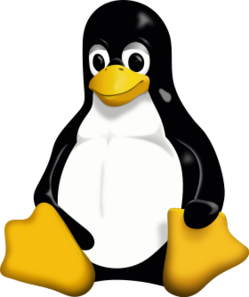
\includegraphics[width=.08\textwidth]{logo-tux.png}\hfill
  
\includegraphics[width=.3\textwidth]{logo-unab.png}\hfill
  
\includegraphics[width=.08\textwidth]{logo-python.png}
}

\makeatletter
\setbeamertemplate{title page}{
  \begin{minipage}[b][\paperheight]{\textwidth}
    \vfill%
    \ifx\inserttitle\@empty\else\usebeamertemplate*{title}\fi
    \ifx\insertsubtitle\@empty\else\usebeamertemplate*{subtitle}\fi
    \usebeamertemplate*{title separator}
    \ifx\beamer@shortauthor\@empty\else\usebeamertemplate*{author}\fi
    \ifx\insertdate\@empty\else\usebeamertemplate*{date}\fi
    \ifx\insertinstitute\@empty\else\usebeamertemplate*{institute}\fi
    \vfill
    \ifx\inserttitlegraphic\@empty\else\inserttitlegraphic\fi
    \vspace*{1cm}
  \end{minipage}
}
\makeatother


\makeatletter
\setlength{\metropolis@titleseparator@linewidth}{2pt}
\setlength{\metropolis@progressonsectionpage@linewidth}{2pt}
\setlength{\metropolis@progressinheadfoot@linewidth}{2pt}
\makeatother


\begin{document}

% ------------------------------------------------------------------------
% Portada personalizada (en tu preamble, podrías haber definido \myfront)
% ------------------------------------------------------------------------
\myfront{}

% ------------------------------------------------------------------------
% SLIDE 1: Título de la sesión (Semana 2, Sesión 1)
% Según el syllabus, esta vendría a ser la "Sesión 3"
% ------------------------------------------------------------------------
\begin{frame}
  \titlepage
  % Ajusta el título/subtítulo si quieres más detalle, por ejemplo:
  % \title{Semana 2 - Sesión 1 (Sesión 3): Sintaxis Básica de Python}
\end{frame}

% ------------------------------------------------------------------------
% SLIDE 2: Índice / Tabla de contenidos
% ------------------------------------------------------------------------
\begin{frame}
  \frametitle{Resumen - Semana 2, Sesión 1 (Sesión 3)}
  \tableofcontents
\end{frame}

% ------------------------------------------------------------------------
% Configuración de bloques (en caso de usar metrópolis, etc.)
% ------------------------------------------------------------------------
\metroset{block=fill}

% ----------------------------------------------------------------------------------------
% SECCIÓN 1: Contexto de la Sesión
% ----------------------------------------------------------------------------------------
\section{Introducción a la Sesión 3}

% ------------------------------------------------------------------------
% Slide 3: Objetivos de la Sesión
% ------------------------------------------------------------------------
\begin{frame}{Objetivos de la Sesión 3}
  \begin{itemize}
    \item \textbf{Abordar} la sintaxis básica de Python de forma más sistemática.
    \item \textbf{Profundizar} en los tipos de datos, variables y operaciones aritméticas.
    \item \textbf{Realizar} ejemplos interactivos en Google Colab para afianzar la comprensión.
    \item \textbf{Fomentar} la colaboración y el trabajo grupal.
  \end{itemize}
\end{frame}

% ------------------------------------------------------------------------
% Slide 4: Conexión con la Sesión Anterior
% ------------------------------------------------------------------------
\begin{frame}{Conexión con Sesiones Previas}
  \begin{itemize}
    \item Sesión 1 y 2 (Semana 1) se enfocaron en:
      \begin{itemize}
        \item Introducción al entorno Google Colab.
        \item Operaciones básicas y entrada/salida en Python.
        \item Ejercicios simples de asignación y aritmética.
      \end{itemize}
    \item Ahora profundizaremos en la \textbf{estructura y sintaxis} de Python.
  \end{itemize}
\end{frame}

% ----------------------------------------------------------------------------------------
% SECCIÓN 2: Sintaxis Básica de Python
% ----------------------------------------------------------------------------------------
\section{Sintaxis Básica de Python}

% ------------------------------------------------------------------------
% Slide 5: Reglas Fundamentales de Sintaxis
% ------------------------------------------------------------------------
\begin{frame}{Reglas Fundamentales de la Sintaxis de Python}
  \begin{itemize}
    \item \textbf{Indentación}: Bloques de código se definen por la sangría (\texttt{4 espacios} usualmente).
    \item \textbf{Uso de dos puntos} (\texttt{:}) para iniciar bloques (if, while, for, funciones, etc.).
    \item \textbf{Sensibilidad a mayúsculas/minúsculas}: \texttt{var} es distinto de \texttt{Var}.
    \item \textbf{Comentarios}: Empiezan con \texttt{\#} en una sola línea o con \texttt{""" ... """} para bloques.
  \end{itemize}
\end{frame}

% ------------------------------------------------------------------------
% Slide 6: Comentarios y Buenas Prácticas
% ------------------------------------------------------------------------
\begin{frame}[fragile]{Comentarios y Buenas Prácticas}
  \textbf{Ejemplo de comentarios en Python}:
  \begin{minted}{python}
# Esto es un comentario de una sola línea

"""
Este es un comentario
que abarca múltiples
líneas de texto
"""

x = 5  # Asigno 5 a x
print(x)
  \end{minted}
  \begin{itemize}
    \item \textbf{PEP8}: Recomendaciones oficiales de estilo (espacios, nombres de variables, etc.). https://peps.python.org/pep-0008/
    \item Facilita la lectura y el mantenimiento de código.
  \end{itemize}
\end{frame}

% ------------------------------------------------------------------------
% Slide 7: Palabras Reservadas y Convenciones
% ------------------------------------------------------------------------
\begin{frame}{Palabras Reservadas y Convenciones}
  \begin{itemize}
    \item \textbf{Palabras Reservadas}: \texttt{if, elif, else, for, while, import, class, def, return, ...}
    \item \textbf{Nombrado de variables}:
      \begin{itemize}
        \item Usar \emph{snake\_case} para variables y funciones: \texttt{mi\_variable}, \texttt{calcular\_area()}.
        \item Mayúsculas para constantes: \texttt{PI = 3.14159}.
      \end{itemize}
    \item \textbf{Longitud de línea}: Idealmente menor a 79 caracteres (conforme a PEP8).
  \end{itemize}
\end{frame}

% ----------------------------------------------------------------------------------------
% SECCIÓN 3: Reforzando Tipos de Datos, Variables y Operaciones
% ----------------------------------------------------------------------------------------
\section{Refuerzo de Tipos y Variables}

% ------------------------------------------------------------------------
% Slide 8: Recordatorio de Tipos de Datos
% ------------------------------------------------------------------------
\begin{frame}{Recordatorio: Tipos de Datos en Python}
  \begin{itemize}
    \item \textbf{int}: números enteros (\texttt{10, -3, 0, 9999}).
    \item \textbf{float}: números con punto decimal (\texttt{3.1415, 1.0, -2.5}).
    \item \textbf{complex}: números complejos (\texttt{3+4j}).
    \item \textbf{bool}: \texttt{True} / \texttt{False}.
    \item \textbf{str}: cadenas de texto (\texttt{"Hola"}, \texttt{'Mundo'}).
  \end{itemize}
\end{frame}

% ------------------------------------------------------------------------
% Slide 9: Revisando Conversiones (Casting)
% ------------------------------------------------------------------------
\begin{frame}[fragile]{Conversiones Explícitas (Casting)}
\begin{minted}{python}
# De string a entero
edad_str = input("Ingresa tu edad: ")
edad = int(edad_str)

# De string a float
altura_str = input("Ingresa tu altura (m): ")
altura = float(altura_str)

# De int a float
numero_entero = 5
numero_flotante = float(numero_entero)  # 5.0
\end{minted}
\begin{itemize}
  \item \textbf{ValueError} si la conversión es inválida (ej.: \texttt{int("hola")}).
\end{itemize}
\end{frame}

% ------------------------------------------------------------------------
% Slide 10: Operaciones Aritméticas y Prioridades
% ------------------------------------------------------------------------
\begin{frame}[fragile]{Operaciones y Precedencia}
\begin{minted}{python}
# Orden de precedencia:
# 1. Paréntesis
# 2. Exponente **
# 3. Multiplicación, División, Módulo
# 4. Suma y Resta

a = 2 + 3 * 4      # 2 + 12 = 14
b = (2 + 3) * 4    # 5 * 4 = 20
c = 2**3 * 3       # 2^3 * 3 = 24
\end{minted}
\begin{itemize}
  \item \textbf{Evitar ambigüedades}: usar paréntesis cuando sea necesario.
  \item \textbf{Operadores compuestos}: \texttt{+=}, \texttt{-=}, \texttt{*=}, \texttt{/=}.
\end{itemize}
\end{frame}

% ------------------------------------------------------------------------
% Slide 11: Actividad 1 - Ejercicios Rápidos
% ------------------------------------------------------------------------
\begin{frame}{Actividad 1: Ejercicios Rápidos en Colab}
  \begin{itemize}
    \item Crea un nuevo \textbf{notebook} para “Semana 2, Sesión 1”.
    \item Implementa ejercicios:
      \begin{enumerate}
        \item Calcular \((3+4) * 2^2\) y mostrar resultado.
        \item Ingresar una cadena y convertirla en \texttt{int} o \texttt{float}.
        \item Usar un \textbf{print} para concatenar texto con variables numéricas.
      \end{enumerate}
    \item \textbf{Tip}: Observa qué pasa si ingresas valores no válidos.
  \end{itemize}
\end{frame}

% ----------------------------------------------------------------------------------------
% SECCIÓN 4: Ejemplos Interactivos en Colab
% ----------------------------------------------------------------------------------------
\section{Ejemplos Interactivos}

% ------------------------------------------------------------------------
% Slide 12: Ejemplo 1 - Manejo de Variables
% ------------------------------------------------------------------------
\begin{frame}[fragile]{Ejemplo 1: Manejo de Variables}
\begin{minted}{python}
nombre = input("¿Cuál es tu nombre? ")
edad_str = input("¿Cuál es tu edad? ")
edad = int(edad_str)

# Jugando con los datos
edad_futura = edad + 5
print("Hola,", nombre)
print("Hoy tienes", edad, "años.")
print("Dentro de 5 años tendrás", edad_futura, "años.")
\end{minted}
\textbf{Discusión}: Manejo de \texttt{int} vs. \texttt{str}, impresiones múltiples.
\end{frame}

% ------------------------------------------------------------------------
% Slide 13: Ejemplo 2 - Aritmética Directa
% ------------------------------------------------------------------------
\begin{frame}[fragile]{Ejemplo 2: Aritmética Directa en Colab}
\begin{minted}{python}
# Aritmética directa en una celda Colab
result1 = (2 + 3) * (5 - 1)
result2 = 10 / 2 + 6 // 3 - 4
print("Result1 =", result1)
print("Result2 =", result2)
\end{minted}

\textbf{Punto a destacar}:
\begin{itemize}
  \item \texttt{//} es \textbf{división entera} (trunca el resultado).
  \item \texttt{/} es división flotante (da decimal).
\end{itemize}
\end{frame}

% ----------------------------------------------------------------------------------------
% SECCIÓN 5: Actividad Colaborativa
% ----------------------------------------------------------------------------------------
\section{Actividad Colaborativa}

% ------------------------------------------------------------------------
% Slide 14: Ejercicio Grupal - Pequeño Desafío
% ------------------------------------------------------------------------
\begin{frame}{Ejercicio Grupal: Mini-Calculadora}
  \begin{block}{Enunciado}
    \begin{itemize}
      \item Crear un programa que simule una “mini-calculadora”.
      \item Se piden dos números (float) y una operación (\texttt{+, -, *, /}).
      \item Se muestra el resultado de la operación.
    \end{itemize}
  \end{block}
  \textbf{Extensión}: Manejar la división por cero con un mensaje de error.
\end{frame}

% ------------------------------------------------------------------------
% Slide 15: Organización de Grupos
% ------------------------------------------------------------------------
\begin{frame}{Trabajo en Grupos}
  \begin{itemize}
    \item Equipos de 2-3 integrantes.
    \item Cada equipo edita un notebook compartido en Google Colab.
    \item Discutir la mejor forma de:
      \begin{itemize}
        \item Pedir los datos al usuario.
        \item Validar la operación.
        \item Mostrar los resultados.
      \end{itemize}
    \item Al final, compararán las soluciones y estrategias.
  \end{itemize}
\end{frame}

% ------------------------------------------------------------------------
% Slide 16: Ejemplo de Solución (Mini-Calculadora)
% ------------------------------------------------------------------------
\begin{frame}[fragile]{Ejemplo de Solución (Mini-Calculadora)}
\begin{minted}[fontsize=\tiny]{python}
num1_str = input("Ingresa el primer número: ")
num2_str = input("Ingresa el segundo número: ")
op = input("Ingresa la operación (+, -, *, /): ")

num1 = float(num1_str)
num2 = float(num2_str)

if op == "+":
    res = num1 + num2
elif op == "-":
    res = num1 - num2
elif op == "*":
    res = num1 * num2
elif op == "/":
    if num2 == 0:
        res = "Error: división por cero"
    else:
        res = num1 / num2
else:
    res = "Operación inválida"

print("Resultado:", res)
\end{minted}
\end{frame}

% ------------------------------------------------------------------------
% Slide 17: Análisis y Dudas Frecuentes
% ------------------------------------------------------------------------
\begin{frame}{Análisis y Dudas Frecuentes}
  \begin{itemize}
    \item \textbf{Uso de if/elif/else}: Estructura básica de control, veremos más en profundidad pronto.
    \item \textbf{Validaciones}: Cómo manejar entradas no numéricas o el caso de división por cero.
    \item \textbf{Buenas prácticas}: Comentar líneas clave, usar nombres de variables descriptivos.
  \end{itemize}
\end{frame}

% ------------------------------------------------------------------------
% Slide 18: Tiempo de Discusión
% ------------------------------------------------------------------------
\begin{frame}{Discusión en Grupo}
  \begin{itemize}
    \item ¿Qué método usó cada grupo para manejar la división por cero?
    \item ¿Cómo presentar un mensaje de error informativo?
    \item ¿Se te ocurrió alguna manera de extender la mini-calculadora? (e.g. potencia, módulo).
  \end{itemize}
  \vspace{0.2cm}
  \textbf{Comparte tus conclusiones con la clase.}
\end{frame}

% ----------------------------------------------------------------------------------------
% SECCIÓN 6: Conclusiones y Próximos Pasos
% ----------------------------------------------------------------------------------------
\section{Conclusiones}

% ------------------------------------------------------------------------
% Slide 19: Resumen de la Sesión
% ------------------------------------------------------------------------
\begin{frame}{Resumen de la Sesión}
  \begin{itemize}
    \item Reafirmamos la \textbf{estructura básica} y reglas de sintaxis en Python (indentación, mayúsculas, etc.).
    \item Exploramos con mayor detalle los \textbf{tipos de datos} y la \textbf{aritmética}.
    \item Realizamos ejercicios prácticos en Colab para afianzar la comprensión.
    \item Desarrollamos una pequeña \textbf{mini-calculadora} colaborativamente.
  \end{itemize}
\end{frame}

% ------------------------------------------------------------------------
% Slide 20: Visión para la Próxima Sesión
% ------------------------------------------------------------------------
\begin{frame}{Próximos Pasos}
  \begin{itemize}
    \item \textbf{Sesión 4 (Semana 2)}: Continuar con \textbf{estructuras de control} (\texttt{if, while}), y ejercicios más complejos.
    \item \textbf{Tarea sugerida}:
      \begin{itemize}
        \item Practicar la creación de scripts con menús (mini-calculadora mejorada).
        \item Revisar la documentación de Python sobre tipos numéricos y funciones matemáticas.
      \end{itemize}
  \end{itemize}
\end{frame}

% ------------------------------------------------------------------------
% Slide 21: Recursos Extra
% ------------------------------------------------------------------------
\begin{frame}{Recursos Extra}
  \begin{itemize}
    \item \href{https://docs.python.org/3/tutorial/}{\textbf{Python Official Tutorial}} (apartados 1-3).
    \item \href{https://realpython.com/}{\textbf{Real Python}} (guías introductorias).
    \item \href{https://peps.python.org/pep-0008/}{\textbf{PEP8 Style Guide}}: Recomendaciones de estilo y formato (útil para mantener código limpio).
  \end{itemize}
\end{frame}

% ------------------------------------------------------------------------
% Slide 22: Breve Ejercicio Adicional
% ------------------------------------------------------------------------
\begin{frame}{Ejercicio Adicional (Opcional)}
  \begin{block}{¡Desafío!}
    \begin{itemize}
      \item Crea un programa que pida el \textbf{radio de un círculo} y elija:
        \begin{itemize}
          \item '1' para calcular el \textbf{diámetro}.
          \item '2' para calcular la \textbf{circunferencia}.
          \item '3' para calcular el \textbf{área}.
        \end{itemize}
      \item Muestra el resultado correspondiente (usa \texttt{math.pi}).
    \end{itemize}
  \end{block}
  \textbf{Comentario}: Requiere condicionales y entradas numéricas.
\end{frame}

% ------------------------------------------------------------------------
% Slide 23: Recomendación para Estudio
% ------------------------------------------------------------------------
\begin{frame}{Recomendación para Estudio}
  \begin{itemize}
    \item Al finalizar la clase, escribe \textbf{notas de lo aprendido} en tu cuaderno.
    \item Identifica \emph{dónde} has tenido más dudas:
      \begin{itemize}
        \item Manejo de strings vs. números.
        \item Operaciones matemáticas.
        \item Orden de ejecución en un notebook.
      \end{itemize}
    \item Prepara preguntas concretas para la siguiente sesión.
  \end{itemize}
\end{frame}

% ------------------------------------------------------------------------
% Slide 24: Retroalimentación General
% ------------------------------------------------------------------------
\begin{frame}{Retroalimentación}
  \begin{itemize}
    \item ¿Te sientes más cómodo con la sintaxis de Python?
    \item ¿Ha quedado clara la importancia de la indentación?
    \item ¿Tienes inquietudes sobre el uso de Google Colab u otro entorno?
  \end{itemize}
  \vspace{0.3cm}
  \textbf{Expón tus dudas e impresiones.}
\end{frame}

% ------------------------------------------------------------------------
% Slide 25: Cierre de la Sesión
% ------------------------------------------------------------------------
\begin{frame}
  \huge{\centerline{¡Gracias y hasta la próxima sesión!}}
  \vspace{0.3cm}
  \normalsize
  \begin{itemize}
    \item Asegúrate de \textbf{guardar tu notebook} en Drive.
    \item Si tienes tiempo, aborda el ejercicio adicional.
    \item Nos vemos en la \textbf{Sesión 4 (Semana 2)} para profundizar en \texttt{if} y \texttt{while}.
  \end{itemize}
\end{frame}

\end{document}

